\documentclass[
  article,                     % Document class
	a4paper,                     % Document size
	12pt,                        % Main text size
	oneside,                     % Only one side of paper
  ]{abntex2}                   % ABNTtex2 for abnt norms

\usepackage[utf8]{inputenc}

% USEFULL PACKAGES ----------------------------------------------
\usepackage{animate}           % GIF images
\usepackage{subfiles}          % Better organization of subfiles
\usepackage[final]{pdfpages}   % Add pdf pages in the work
\usepackage{enumitem}          % Best enumetare
\usepackage{polyglossia}       % Language package
\usepackage{tikz}              % Draw package
\setdefaultlanguage{english}   % Default document language
\SetLanguageKeys{english}{indentfirst=true}
% ---------------------------------------------------------------

% SECTION TITLE FORMAT AND TOC ----------------------------------
\usepackage{titlesec}
\usepackage{titletoc}
% ---------------------------------------------------------------

% FONTS CONFIGURATION -------------------------------------------
\usepackage[no-math]{fontspec} % Add new fonts in document
\setmainfont{Times New Roman}  % Main font of the document
% ---------------------------------------------------------------

% PARAGRAPHS ----------------------------------------------------
\usepackage{parskip}		       % Space in between paragraphs
\usepackage{microtype} 	       % Improves general appearance
% ---------------------------------------------------------------

% MATH ----------------------------------------------------------
\usepackage{newtx}             % Math times new roman font
\usepackage{amsmath}           % Add many configurations in the math space 
\usepackage{bm}                % Bold mathematics 
% ---------------------------------------------------------------

% IMAGES, POSICIONING AND LEGENDS -------------------------------
\usepackage{tabularx}          % Add better tables
\usepackage{subcaption}        % Add a subcaption for figure
\usepackage{float}             % Make the image fixed [H]
\usepackage{multicol}          % Multiple columns text
\usepackage{multirow}          % Multiple rows text
\usepackage{longtable}         % Tables oversized
% \usepackage{graphicx}          % Add better figures
\graphicspath{{images/}}
% ---------------------------------------------------------------

% HYPERLINKS, METADATA AND PROGRAMATION -------------------------
\usepackage{hyperref}          % Create hyperlinks
\usepackage{listings}          % Create algorithms
% \usepackage{minted}
% ---------------------------------------------------------------

% EXTRA MATH SYMBOLS JUST BECAUSE -------------------------------
% Define bold symbols for vectors and matrices
% NOTE: DESNECESSÁRIO, EU SEI, MAS O CHAT ADAPTOU AS EQUAÇÕES E NÃO QUIS PERDER TEMPO CRIANDO SENTIDO NAS LOUCURAS DA IA :)
\newcommand{\mat}[1]{\mathbf{#1}}
\newcommand{\vecc}[1]{\mathbf{#1}}
% ---------------------------------------------------------------

% REFERENCES AND CITATIONS --------------------------------------
\usepackage[
  style=abnt,
  language=english, 
  repeatfields,
  backend=biber,
  useprefix=false,
  extrayear
]{biblatex}
\usepackage{csquotes} % Used for multiple languages styles
\addbibresource{references.bib} % Add here your .bib archive
% ---------------------------------------------------------------

% COVERS DATA ---------------------------------------------------
\orientador{Simone dos Santos Hoefel, Ph.D} % Professor name
\titulo{ANALYSIS OF PASSIVE VIBRATION MITIGATION AND BAND GAP LOCALIZATION IN TLP TENDONS USING A PERIODICALLY SEGMENTED EULER-BERNOULLI BEAM MODEL} % Title
\autor{DÁRIO CARVALHO VIVEIROS} % Author name
\local{TERESINA $-$ PI} % Local
\preambulo{This work was presented to the Center of Technology (CT) of the Federal University of Piauí (UFPI), as a requirement for obtaining the degree of Bachelor in Mechanical Engineering.} % Work nature text
% ---------------------------------------------------------------

% CHANGES THE NAME OF CAPTIONS AND SECTIONS ---------------------
% Add some text here to change values for English text and leave empty for Portuguese text
\def\english{on}
% ---------------------------------------------------------------

% ADDITIONAL PACKAGES AND USEFULL SETUPS FOR PACKAGES -----------
\usepackage{configDir/configurations}
% ---------------------------------------------------------------

\begin{document} % DOCUMENT 

% COVERS AND PAGE NUMBERING -------------------------------------
\pagenumbering{gobble}\covercontent\newpage % Cover
\pagenumbering{arabic}\backcovercontent\newpage % Back cover
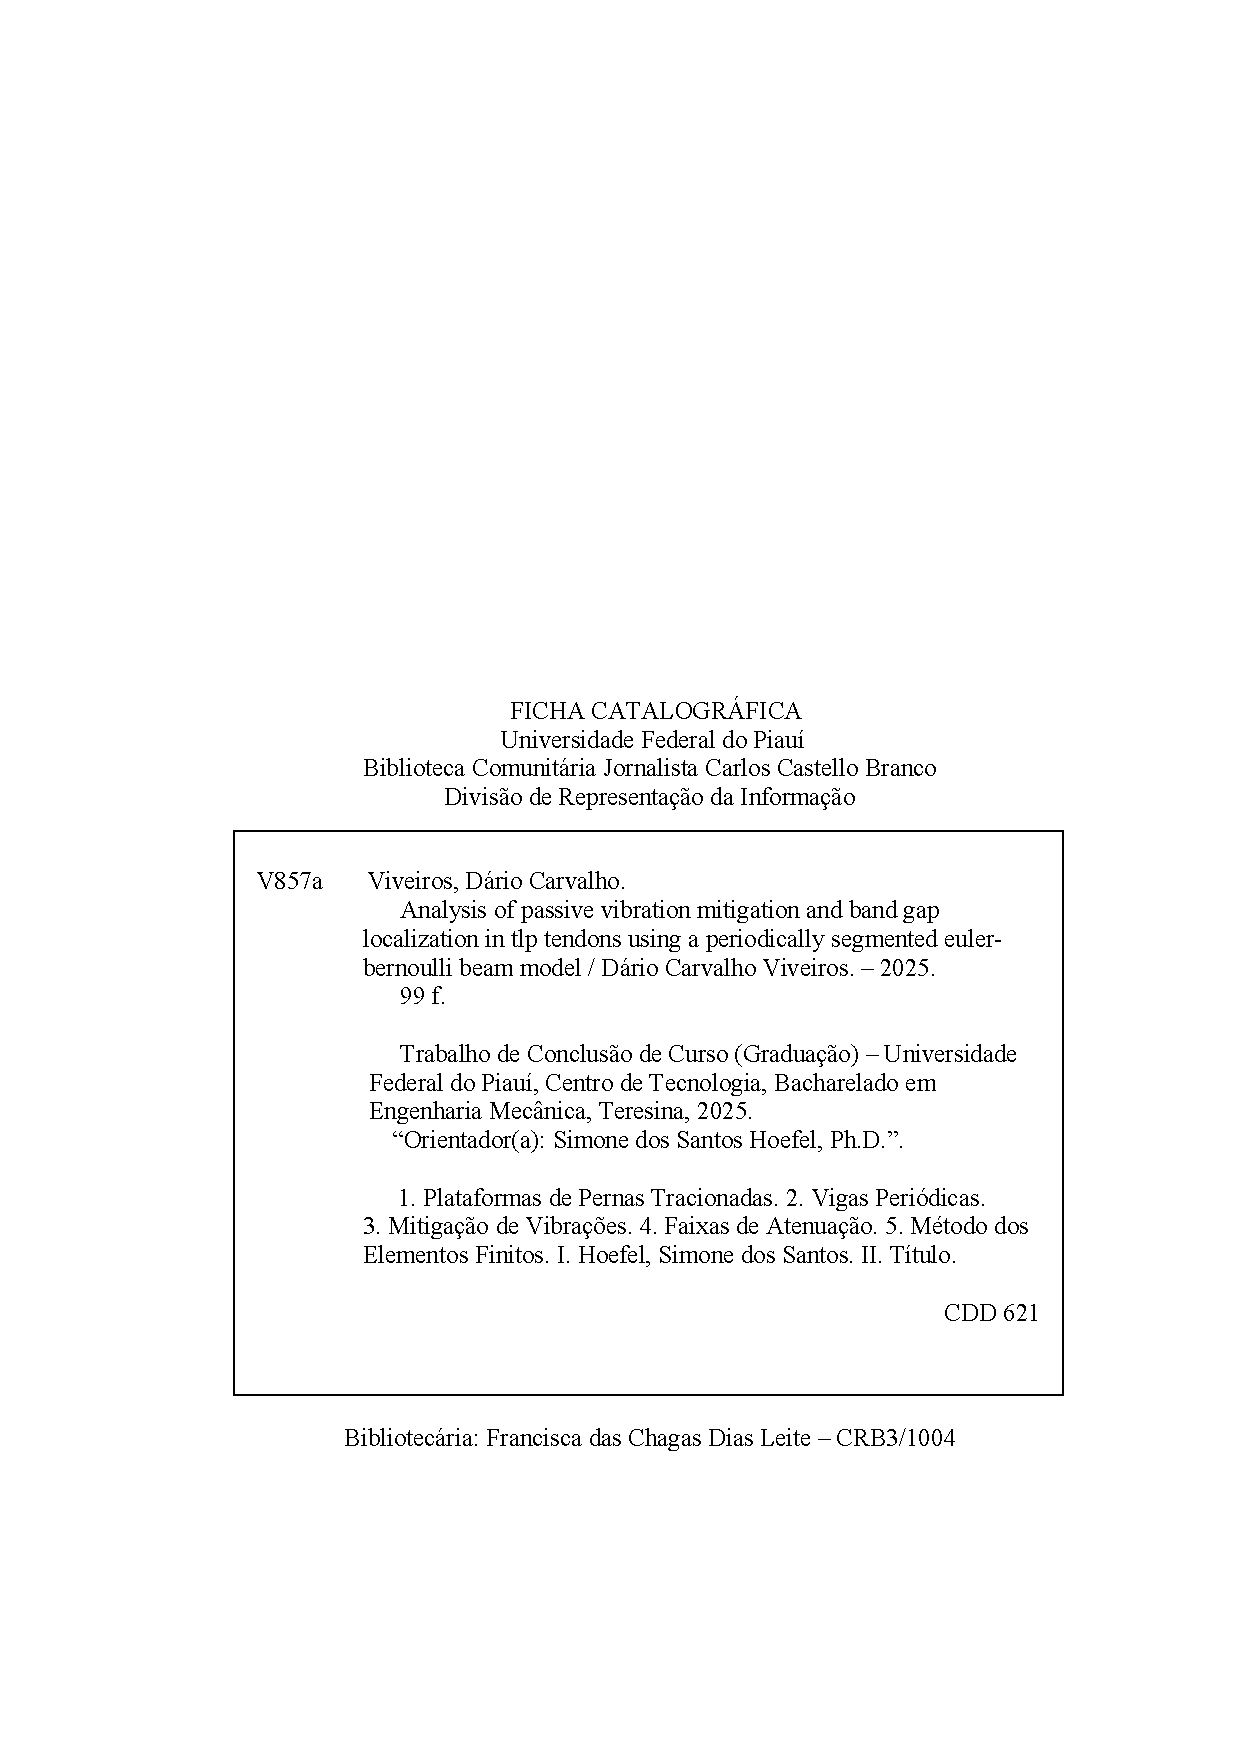
\includepdf[pages=-]{ficha_catalografica_581246.pdf} % Catalog Card
\aprocovercontent\newpage % Approval cover

% TEXTUAL SPACING -----------------------------------------------
\setSpacing{1.5} % Text spacing

% DEDICATION AND ACKNOWLEDGMENT AND EPIGRAPH --------------------
\subfile{acknowledgment}\newpage

% ABSTRACT ------------------------------------------------------
\subfile{Textual/01_vernacular_abstract}\newpage
\subfile{Textual/02_abstract}\newpage

% LIST OF FIGURES AND TABLE -------------------------------------
\listoffigures* \newpage 
\listoftables* \newpage
% \subfile{Textual/03_list_of_acronym}\newpage
\subfile{Textual/04_list_of_variables}\newpage
% SUMMARY -------------------------------------------------------
\tableofcontents*\newpage

% TEXTUAL SPACE -------------------------------------------------
\textual % Textual start 
\pagestyle{simple} % Header and footer style

% TEXTUAL ELEMENTS ----------------------------------------------
% \subfile{instructions.tex}
\subfile{Textual/05_introduction}
\subfile{Textual/06_objective}
\subfile{Textual/06.5_background}
\subfile{Textual/07_methodology}
\subfile{Textual/08_results}
\subfile{Textual/09_conclusion}

% REFERENCES ----------------------------------------------------
\newpage\phantomsection
\addcontentsline{toc}{section*}{\normalfont\bfseries \referenctitle}
\printbibliography[title={\centering \referenctitle}]

% APPENDICES AND ANNEXES ----------------------------------------
\subfile{Textual/10_appendix}
% ---------------------------------------------------------------

\end{document} % DOCUMENT 